\documentclass[14pt]{report}
\usepackage[utf8]{inputenc}
\usepackage{blindtext}
\usepackage{amsmath}
\usepackage[margin=1in]{geometry} 
\usepackage{graphicx,changepage}
\usepackage{xcolor}
\usepackage{hyperref}
\usepackage{tcolorbox}
\usepackage{subfig}
\usepackage{fancyvrb}
\usepackage{listings}
\usepackage{svg}
\usepackage{dirtytalk}
\usepackage{csvsimple}
\newcommand\todo[1]{\textcolor{red}{#1}}
\title{Legend Of Bluespec}
\author{kr469 }
\date{October 2021}

\tcbset{colback=pink!7,colframe=pink!90,coltitle=black}
\begin{document}

\maketitle
\tableofcontents

\chapter{Introduction}

Making hardware is hard, and similarly to other problems in computer science, we make it easier by adding layers of abstraction. There are many layers involved in making hardware from that abstract transistors to gates to logical operations to functions to modules to chips to multi-chip modules to whole devices. The layer this project focuses on is going from modules to chips(TODO: this probably need renaming, add graph showing layers). At this layer we already have code for modules like memory, CPU-cores, interconnects and so on. Now what we need is an ability to compose them in such a way that they create a whole device.

\section{Motivation}
\begin{tcolorbox}[title=Vocabulary]
    \begin{itemize}
        \item Verilog - Hardware description language
        \item Bluespec - Hardware description language
        \item Intel Quartus Prime (IQP) - programmable logic device design software produced by Intel. (source Wikipedia)
        \item Platform Designer - Tool inside IQP used to connect high level components.
    \end{itemize}
\end{tcolorbox}
Verilog is an old language with minimal type system. This forces people to encode more complex interfaces using finicky naming conventions. To simplify process of connecting components with many wires, people tend to use high level tools like Platform Designer, that have built in logic allowing for easy connection of components. This approach is not perfect and as we will see during evaluation, a better option might be to move away from Verilog and to use more modern language like Bluespec. The problem with that is that tools like Intel Quartus Prime(IQP) don't have native support for Bluespec, and it forces Bluespec users to work with transpiled Verilog (from Bluespec) code. Unfortunately, because typing richness of Bluespec(comparable to Haskell), arbitrary code cannot be transpiled, and before code can be transpiled it needs to be stripped of any arguments or other kinds of polymorphism. Process of transpiration also destroys high level interfaces, and they must be recreated manually after importing Verilog code into IQP. 

\section{Already existing tools}
Creating custom hardware has got expensive in last few decades both in therms of money but also in terms of man-hours needed to create it. 
This creates barriers to entry for new players, and also reinforces strong positions of already adopted standards. 
This also means that there isn't as large open source community as around hardware and therefore one cannot simply use plugin for Bluespec of Bluespec native high level integration tool because there are none.

My project will try to tackle a subset of functionality provided by a tool called Platform Designer that is a part of Intel Quartus Prime package. Platform Designer is a GUI tool for high-level integration, designs generated by it are kept in verbose text file format. Unfortunately, those files have a tendency to be megabytes long, making them hard to read and edit, by humans. There are other problems with using Platform Designer, like cumbersomeness of importing new components.

\begin{tcolorbox}[title=Market share and justification for focusing entirely on comparisons with Intel Quartus Prime]
    It's a bit difficult to accurately judge market share of IQP, but It is produced by one of the biggest designer and manufacturer in the world, and it's also used by Qualcomm according to \href{https://discovery.hgdata.com/product/intel-quartus-prime}{HG Insights}. Using Google trends we can see that while in recent years(since 2016) competitor Xilinx Vivado has overtaken, IQP in interest at the global scale, in most developed countries like US, Europe, and parts of Asia. There is roughly 50/50 split between IQP and Vivado. My personal observations suggest that Xilinx Vivado became highly popular in India which is a large country with history of chip design, and this might be strongly skewing data in favor of Xilinx's product. Another argument to compare against IQP is that it was used last year as a part of the course, and it can't be irrelevant if it was taught at Cambridge. Therefore, it's fair to not investigate Xilinx's software during evaluation(TODO: check if this has changed).
\end{tcolorbox}

\section{Proposed solution}
During my project I created an alternative JSON based file format that is much simpler and human-readable, that can be interpreted using my tool to produce Bluespec code of a top level module.
This file format is rather unimpressive on its own, and one might argue that it would be better to use Bluespec code instead of it. Interesting part of this project lie in the backend that is able to verify correctness of this file and produce set of typing information about produced Bluespec code.
But to truly appreciate work I have done during this project I also implemented GUI, which uses same backend as one used to interpret JSON files, and it is able to supply user with typing information and possible choices when connecting components. 
One can think of it as a Bluespec native high level integration tool that uses simple language server in the backend. This way Bluespec user can do high level integration in the realm of not transpiled Bluespec. Then after satisfactory top level module is created, it can be transpiled to Verilog and then imported into IQP.

\chapter{Preparation}

\section{Understanding Bluespec}
Before I started this project my only knowledge about Bluespec was from \href{https://www-bluespec.cl.cam.ac.uk/}{Cambridge Bluespec Tutor} which covers basics, and It was completed by me few weeks prior to the start of this project. For the purposes of understanding this project I've learned about most of the typing system of Bluespec, but for You the reader most of it is not relevant. Therefore, I prepared a short tour of things that will be important to understand in this project. 
\subsection{Rules}
 In Bluespec all computation is done in form of rules. Each cycle we will take a subset of all rules that we are going to execute in this cycle, rule is fired (executed) in cycle only if it's ready (or will be ready) and it's not conflicting with other rules (If this happens compiler must issue a warning, and picks arbitrary rule to fire from subset of conflicting rules). Each rule can fire at most one time per cycle. For rule to be ready to fire it needs it's implicit and explicit conditions to be true. Rule can be fired in a cycle even if it's not ready at the start of cycle, for example if you add item on an empty queue and then pop can happen in same cycle. \\
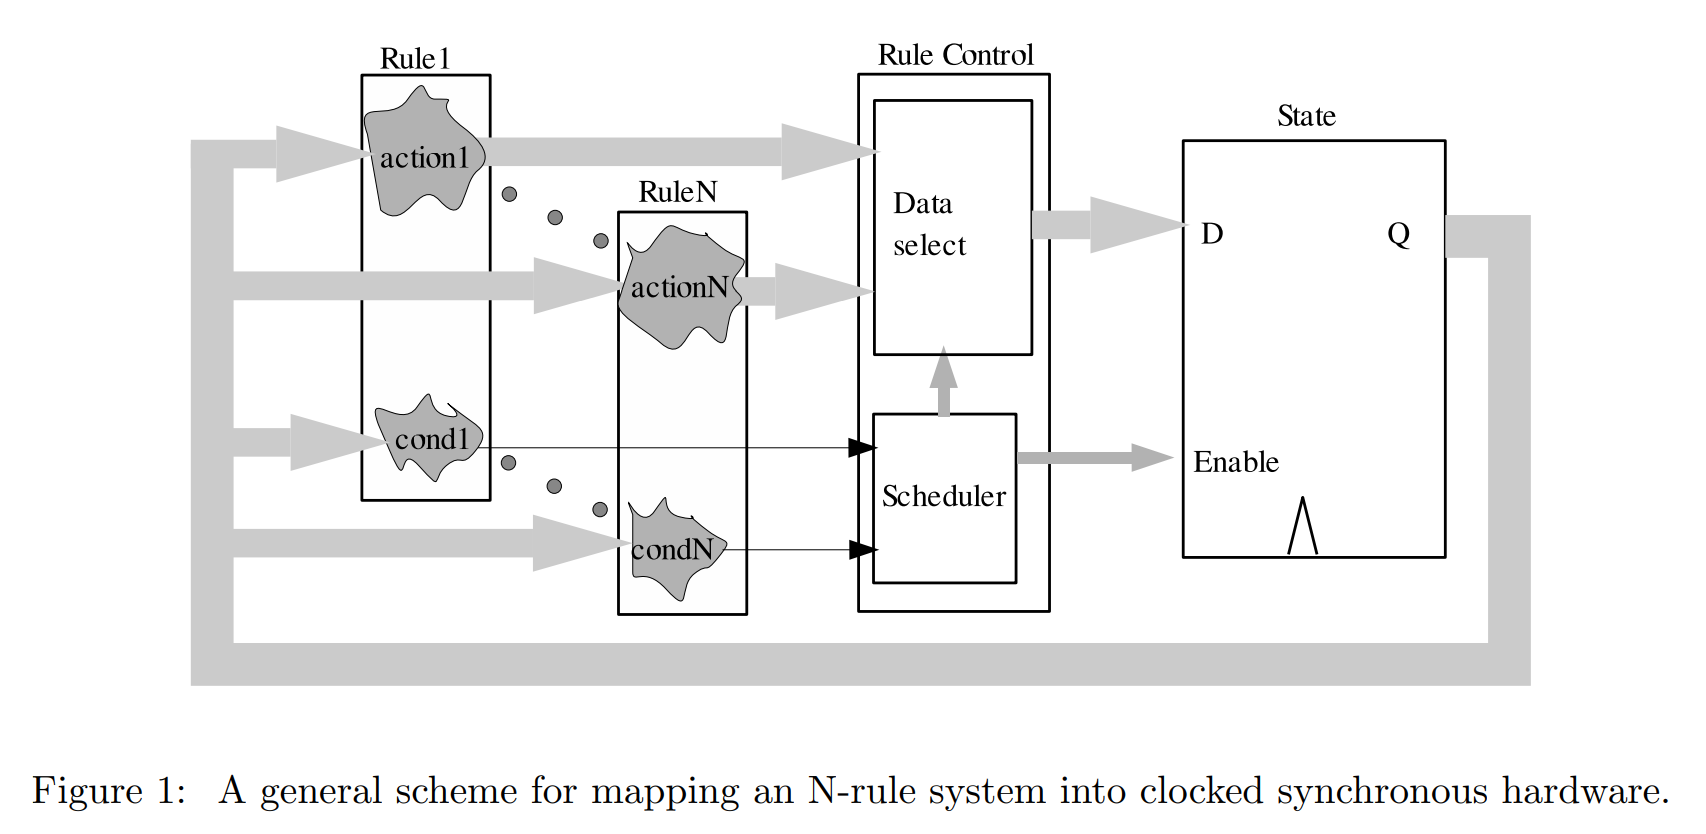
\includegraphics[width=\textwidth]{Rulemapping.png}
(TODO: add reference to the bsv reference document from which this image was taken)
\begin{verbatim}
        
    TODO: piece of Bluespec with module using fifo and other rule
     explaining types of conditions.
    
\end{verbatim}

\subsection{Modules and interfaces}
Module is unit of organization of logic. Modules don't have types, instead they implement some interface. This means that you can have multiple modules with different behaviour that implement the same interface. It might be helpful to think about similarly to different physical connectors(like USB-C, PCI-e). Interfaces are made up out of two types of things:
\begin{itemize}
    \item Methods - that allow for interaction with the module, they come with few variants, but this is not important for now.
    \item Subinterfaces - That allow for more generalization, for example if you want to implement module that contains two copies of the same interface, you can just create a new interface that contains two instances of that subinterface and assign them accordingly.
\end{itemize}

\subsection{Typeclasses}
Typesclasses in Bluespec are used to group types for which specific functions or modules are implemented. Typeclass instance is (TODO describe what is it) and it can have provisos attached to it.

\subsection{Provisos}
On big feature of Bluespec typing is support for provisos. They create constraints on types that can be used with given function and give information about expected type of output of the function. For example, we can have a polymorphic function \verb!extend! of a type \verb!Bit#(a)! $\rightarrow$ \verb!Bit#(b)! where \verb!Bit#(x)! is a vector of $x$ bits, such function accepts any length and always return vector of length $b=a+1$. To make sure this relations stays like this we would attach a proviso \verb!Add#(a,1,b)! which means that $a+1$ must be equal to $b$. 
\par
Mentioned above \verb!Add! is one of Size Relationship provisos, other such provisos are \verb!Mul Div Max Min Log!.
Those provisos can't be nested, but we still can express complex arithmetic constraints, thanks to size relationship type functions.
They essentially represent result of the operation on values on that were supplied. There are only 8 of them, and they are \verb!TAdd TSub TDiv TMul TMax TMin TLog TExp!.
To better explain this let's look at some simple example: \\
\verb!Add#(TExp#(a),TDiv#(a,8),c)! is a proviso that says that following equation on parameters must be satisfied $2^a+\lceil\frac{a}{8}\rceil = c$ otherwise it will mean that supplied parameters are not valid. Those equations can be also solved to deduce unknown parameters.
\par
There is also other type of provisos that are typeclass based.
Typeclass based provisos, allow us to either to ensure certain functions are defined for given type or to deuce something. For example \verb!Bits#(a,b)! means that type \verb!a! must be convertible to vector of $b$ bits. This can be used to get the length in bits of given objects, on which we can later put constraints using Size Relationship provisos.
\\
In my project I will often check if there exists instance of the \verb!Connectable#(a,b)! typeclass to check if function \verb!mkConnection!(used to connect two interfaces together) is defined for given types \verb!a! and \verb!b!.

This can be a bit confusing, but if one look closely this is very similar to Prolog. We have variables that are effectively the same as in Prolog, we have values that are integers, and we have parametric types /functions that are like Prolog's compound terms. Typeclass are like groups of rules with same name and provisos attached to Typeclass instances are like predicates.
One big difference is that provisos can be solved in arbitrary order, which means that unlike in Prolog we need ability to solve sets of equations on integers.


\section{Choosing tools}
I had effectively 3 choices for a language to this project in. Here is some justification why I have chosen Python. 
\subsection{Haskell}
Compiler of Bluespec is written in Haskell. Therefore there are seweral reason why Haskell would be right choice. Here are some of them:
\begin{itemize}
    \item I can reuse already written logic.
    \item I won't diverge in terms of logic from Bluespec compiler.
    \item I won't need to write grammar to load packages.
\end{itemize}
But there are also few very good reasons why I didn't used Haskell.
\begin{itemize}
    \item I never used Haskell before, and my experience with functional languages equal to what was shown in the foundations of the computer science course.
    \item I never used Bluespec before, and my experience is limited to completing Bluespec tutor provided by computer science department.
    \item Even if I knew Haskell and Bluespec, industrial compilers are rather large and complicated. I also received advice to avoid modifying / extending them as a part of the project.
\end{itemize}
While each of those reasons on its own is something that can be managed. All of them combined would create unacceptable amount of risk of not delivering the project. There was also a risk that use of Haskell wouldn't create a good story for the project. (This is quite subtle).

\subsection{Tcl (pronounced "tickle")}
This language is used as a scripting language in both Intel and Xilinx tools, While I will be reading packages using Tcl scripts provided by the creators of the Bluespec compiler (BSC), my understanding is that those scripts are just handy wrappers for some Haskell functions. This is also foreign language to me with minimal presence online, and negligible learning resources, making it difficult to learn. It's also quite obsolete and there is not much tooling for it making it undesirable as a time investment(As an example of desirable to learn technology. I learned for this project JavaScript, just to create a GUI).
\subsection{Python}
Firstly this is a language I have experience working with, secondly it's widely supported, and there is extensive tooling for it. It's flexible typing system allows for rapid experimenting, which was especially handy when I wasn't sure how structure of the data would look like. It's also worth mentioning that it has support for typing and at some point I decided to started adding typing hints around. My rule of thumb that I used was that if Pylance (python language server) can't deduce type of something I need more hints.
Other reasons for using python are:
\begin{itemize}
    \item I will have many interesting problems to solve. Like creating and interpreting grammar.
    \item Code written in it can be used by large community of python developers.
    \item I can use many tools like, Lark (for grammar), Django (as a backend server), SymPy (to solve size relationship provisos) that will speed up the process.
\end{itemize}
The two arguments against using python are:
\begin{itemize}
    \item Haskell would be better suited for this task. I explained above why it doesn't make sense for me to use Haskell. 
    \item Python is usually slow. Fortunately this isn't a big issue thanks to cashing and use of PyPy (implementation of Python using JIT compiler).
\end{itemize}
\subsection{Postmortem}
Looking at those choices now(after finishing project and knowing all encountered difficulties) I think a could also consider \verb!C#!, due to its speed and similar typing flexibility to Python. I also think Haskell would be a better choice if this was more like my pet project on which I would work for few years with the intention of making it commercially viable product.

\section{Creating a grammar}
This section could be moved into implementation.

\begin{tcolorbox}[title=Bluetcl]
    Bluetcl is a tool written in Tcl language that allows for inspection of Bluespec packages. It's a first party tool that included with Bluespec compiler. There isn't much documentation about it, but from my understanding it's a wrapper around Haskell code.
    From the user perspective it's just a bash script that starts Tcl terminal compiled with some libraries. From my perspective I use it as an arbitrary command line program, as this method of using is intended by the authors and contains some documentation.
\end{tcolorbox}
\subsection{What grammar is needed ?}
Because I'm using Bluetcl as a command line tool, communication with it is done via text. 
While synthesizing commands is easy, parsing outputs is a bit more difficult, and I decided to do it in systematic way. 
To do this I need grammar of all possible outputs that I'm interested in. 
Bluetcl produces range of outputs but two of them that are particularly useful are descriptions of functions and descriptions of types.
\subsection{Where to find this grammar ?}
Unfortunately this grammar is not documented anywhere, so I had to reverse engineer it. This approach might not be perfect and might not cover every input, but It's good enough to parse every standard package and every package used to compile Flute(RISC-V CPU with 5 stage pipeline).
Here are other reasons to justify this approach:
\begin{itemize}
    \item Heaps' law suggests that number of unique words in given body of text is proportional to roughly square root of number of words in the text. I think it's fair to assume that something similar will be true if we consider number of unique grammar rules.
    \item This grammar while different from grammar of Bluespec language maps subset of Bluespec grammar, so we can supplement our deductions with reference guide for Bluespec language. Therefore, accounting for cases we haven't seen, but are possible.
    \item There is also some limit on how exotic things can get in top modules. (TODO rephrase this)
\end{itemize}

\subsection{Technical aspects}
This is EBNF grammar, I parse it using Lark library for Python, and I'm using Earley parser, as it is capable of arbitrary length lookahead. Grammar I created contains roughly 90 rules, and I won't include all of them here, but I will show few examples to give a feel of what is happening. (TODO: Think about dumping them into an apendix) 
\\
A useful feature supported by Lark is ability to have regular expressions in the grammar, I'm mentioning this as it is effectively having parser inside a parser. It's also worth mentioning that there exists a handy tool for debugging and creating grammar. It's located at this website: \href{https://www.lark-parser.org/ide/}{https://www.lark-parser.org/ide/}, it can run parser online, and show outputed AST tree.
\begin{tcolorbox}[title = Parsing position TODO maybe find a better example with shorter line]
    Here is an example of parsing small section of output that describes location of piece of code that is being described. I decided to show it as it's simple and shows different features of that I needed to use.
    \begin{verbatim}
-------- Rules used ------------
identifier_u: /[A-Z][\w$_']*/

tcl_position: "{" "position" "{" tcl_path NUMBER NUMBER 
 ["{" "Library" identifier_u "}" ]"}""}"

tcl_path: ["%/"] /((\.{1,2})|(\w|-|\s)+)/ 
 ["/" /((\.\.)|(\.)|((\w|-|\s)+))/]* "." /\w+/

-------- Text to parse ---------
{position {%/Libraries/Connectable.bs 25 1 {Library Connectable}}}
    \end{verbatim}
    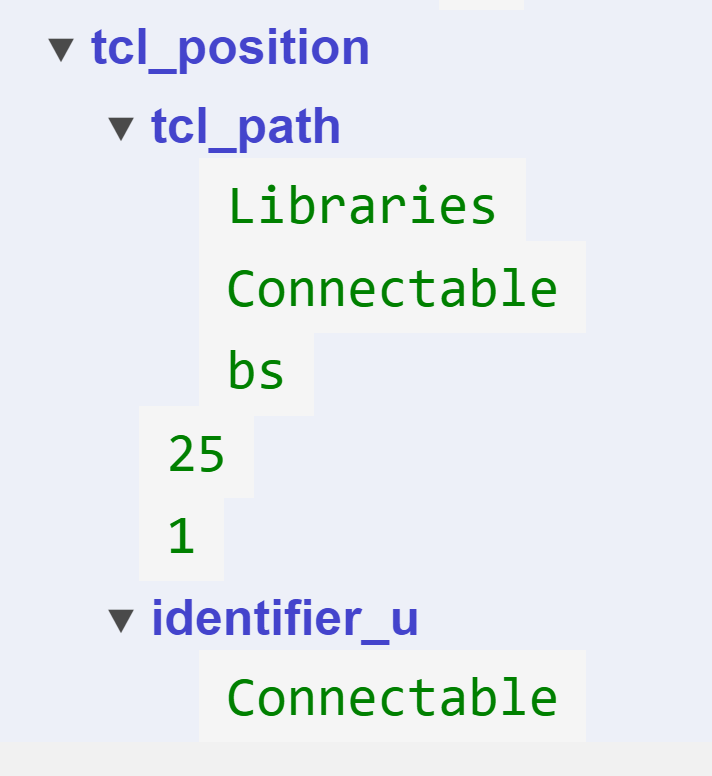
\includegraphics[width=0.4\textwidth]{images/TCLPath.png}
\end{tcolorbox}


\chapter{Implementation}
\section{Reading descriptions of packages}
\subsection{HandlerV2.py Todo rename}
To interact with Bluetcl I have written a script using Pexpect library. This script works by creating subprocess of Bluetcl, and exposes functions that allow for performing of quarries. Core of this script is a function called \verb!call! that takes as input a string that is a command and returns output of stripped of warnings or raises an exception if error occurred(for example in case where package was not found). To remove warnings I make some assumptions.
\begin{itemize}
    \item I only use fixed set of commands(like list packages, describe a type).
    \item For those commands important output about is always on the last line. (this was checked empirically)
    \item Output of a command is always followed by $\%$ a character that never occurs in the rest of the output and marks the end of the output.
\end{itemize}
Thanks to them, I don't need sophisticated system for parsing error, and or warnings. I can just make a quick search for error, and if needed forward this to user.
\\ 
In total this script allows me for:
\begin{itemize}
    \item Initialize subprocess
    \item Add folder to search path of Bluetcl
    \item Load package (Bluetcl takes care of finding and loading dependencies)
    \item Get list of loaded packages
    \item List functions in package
    \item List types in package
    \item Get information about types and function in the package
\end{itemize}

\section{Loading Bluespec packages' information (TODO check grammar of s')}
As mentioned earlier output of bluetcl is text, and I need it in some better organized form. In this section I describe process of doing this.
\subsection{Lexical and syntax analysis}
I decided to use Lark library for lexical and syntax analysis. This library takes grammar and string of text as input and returns an abstract syntax tree. The only difficult part here to create a grammar that works. (TODO improve this last sentence)

\subsection{Understanding abstract syntax tree (AST)}
Given AST I needed to turn it into a more useful form. To do this I used \verb!Transformer! class provided by Lark. The way it worked is that I created subclass of \verb!Transformer! that implemented a function for each non-terminal / rule(Each non-terminal can have multiple rules and Lark allows for renaming individual of rules, this for example allows parsing different non-terminals using same function or parsing single non-terminal using different function depending on rule that was used). \verb!Transformer! will then perform bottom up transformation of AST, and for each rule it will call respective member function, with parsed children(non-terminals used by rule) as arguments. At the end of the transforming process I have a list of objects that represented data from Blutecl.
\\
One of the bigger inconveniences I encounter is the fact that Lark passes parsed children, as a simple list. This doesn't provide information about what exactly each child is, this isn't a problem if rule contains fixed number of non-terminals, but otherwise I employ mix of length based inference, and wrapping of data from children into tuples, to provide remove ambiguity.
\\
What was quite useful at this stage is Python's type system flexibility, I was able to gradually build up \verb!Transformer! class and add typing information only after I had firm understand what type something needs to be. For some things it wasn't immediately obvious, what is the best way to represent them, and what often happen is I would first leave them as lists of unparsed things. Then after I got to the point where I needed to use them I would decide what is an optimal way to represent them.

\subsection{Organizing data and functionality}
I created a class called \verb!TypeDatabase! that provides simple functions that manage loading and parsing packages information. It is also capable of loading and storing it's state to pickle file. This saves a lot of time as all this parsing and communication with bluetcl isn't particularly fast. This class is also a home to set of functionality used to resolve types. From my testing it takes about 370s to load roughly 250 packages that I found included with Bluespec compiler and created to compile Flute CPU. Loading those packages from cached files takes only few seconds.

\section{Building the top level module}
Building the top level module can be broken down into few operations.
\begin{itemize}
    \item Instantiating new modules.
    \item Connecting modules using \verb!mkConnection! function.
    \item Connecting modules using busses.
    \item Synthesizing Bluespec.
\end{itemize} 
Those operations if implemented naively would be almost as simple as formatting a string. But If this was the only thing that this project provided I wouldn't need to go through all the trouble of parsing Bluespec grammar, and generally users would be better off just writing Bluespec code. My unique value proposition is running something similar to a language server, that will be capable of dynamically resolving types, and aiding user in the design process by providing possible connections, informing whether values passed to initialize module are correct, and informing about subinterfaces that can be found in the instantiated modules. 
At the basis of all those features will be type resolution, and I will first explain how it works.
\subsection{Resolving types}

\subsection{Resolving types (implementation)}
In my code there are 4 main functions that combined allow for type resolution:
\begin{itemize}
    \item \verb!merge! function takes two type identifiers and returns map (dictionary) from names of variables to theirs values. It's similar to Prolog's unification operator.
    \item \verb!applyVariables! function takes a dictionary and a type and returns a type with all variables replaced by their values. This is more of a utility function.
    \item \verb!resolveTypeclass! function that takes a type identifier that is an instance of a typeclass and returns dictionary of resolved variables. In Prolog this is like looking which rule can be applied and returning result of applying that rule.
    \item \verb!solveProvisos! function that takes a dictionary and a list of provisos and returns a dictionary with variables. This is like checking predicates in Prolog.
\end{itemize}
Those functions can also fail with exception if something is impossible / wrong data is provided.

Type identifier is a tree where every non leaf node is another type identifier, and leaf nodes are either variables or values(strings, ints). Example type identifier \verb!Foo#(a,42,"file.hex")! is a type with name \verb!Foo! and three arguments \verb!a! (variable) and \verb!42! (int value) and \verb!"file.hex"! (string value). Type identifiers can also describe functions, and those just need to run unification on both result and arguments of a function.

\subsubsection{Merge function}
This function works like a two synchronized dfs's, that go through the trees (type identifiers) and apply logic based on nodes that are beginning currently visited.
This function needs to account for quite a lot of special cases here are some of them:
\begin{itemize}
    \item If one of the nodes is a variable, and other is a value or another type identifier, then we can add such pair to the dictionary of resolved variables.
    \item If both nodes, are type identifiers, we run merge recursively on pairs of theirs children. We also check if type identifiers share the same name.
    \item If one of the nodes is a value, then other node must be either a value with same value, or a variable.
\end{itemize}
The most complicated case is when both nodes are variables. There is a breakdown what happens then. 
\begin{itemize}
    \item Case 1 - Both variables have a value, so I need to check if value is the same.
    \item Case 2 - One of the variables has a value, and other variable doesn't value assigned. In this case I can just copy reference to a value to the other variable.
    \item Case 3 - Neither of the variables has a value. In this case I create a new dummy object and give reference to it to both of the variables. Using references makes it so resolving value of one of the variables will resolve all of them. 
\end{itemize}
If done carefully, this is quite efficient as we don't need to manage propagation of values of variables, everything is done by just writing to shared object.

\subsubsection{Apply variables function}
This function is quite simple, it just traverses a type identifier and replaces all variables with their values.
\subsubsection{Resolve typeclass function}
Earlier, I compared typeclass to groups of Prolog rules with the same name, one thing I didn't mention that typeclasses can also contain something called dependencies, they are something like marking inputs and outputs in Prolog. Those dependencies are used in typeclasses like \verb!Bits#(a,b)! which are used to determine something, and they make sure that resolution of a typeclass is always unambiguous. \\
For example, \verb!Bits#(a,b)! has a dependency \verb!a determines b! which means that you can use it to determine \verb!b! from \verb!a!, but if you know only \verb!b! then you can't use it to determine \verb!a! because there may be multiple types that can be packed to the bit vector of the same length \verb!b!. (TODO check use of 'the' in last sentence)
\\  
To check if proposed instance of a typeclass is a valid instance we perform following algorithm:
\begin{enumerate}
    \item Check if a proposed instance of a typeclass is an instance of a known typeclass, otherwise fail.
    \item If dependencies for a typeclass are defined check if information provided within proposed instance is enough to satisfy one of them.
    \item Iterate over all templates of an instance of a typeclass, then attempt to merge function between a template and the proposed instance. 
    \item If merging failed, jump back to step 3 and continue iteration.
    \item If merging succeeded, attempt to solve provisos.
    \item If provisos were successfully solved, return the dictionary of resolved variables, otherwise continue iteration.
    \item If all iterations failed, fail.
\end{enumerate}
This procedure is a bit slow, so I speed it up by creating look up dictionaries that take as a key a dictionary and as a value a typeclass instance. This method can cut down search time significantly, but there are still rules that use polymorphic functions and those can't be preprocessed away so easily, therefore I call them universal instances and search through them every time. While I could invent many heuristics to speed up this process in general this is still as difficult as halting problem.

\subsubsection{Solve provisos function}
As established earlier, provisos can be of two types, one are based on typeclasses and those can be resolved using above described function, and the other ones are size based and require solving sets of equations on integers. To do this I use library called SymPy. SymPy is a symbolic math library that can be used to solve equations on integers. All I need to do is convert set of provisos into set of equations, and then extract data and put it back into dictionary used to store variables. 

One big problem is that order in which provisos must be solved is not defined, so I handle this by creating set of provisos to be solved. Then I repeatedly iterate over this set and remove solved provisos. If set didn't change after iteration, and it's not empty this means not further progress can be made and raise an exception.

\subsubsection{How those functions can are used}
Thanks to those functions, I can tell user what values can be put into each argument in a function. I can check if arguments passed to a function satisfy provisos when combined. I can give user a list of all possible connection that can be made. 

\section{Synthesizing}
The main goal of the project is to be able to take a JSON with some data and synthesize a top module in the Bluespec language from it. This goal is more like a justification to create a language server like API. With this approach I have some simple core goal, but in the later sections we will see how thanks to all the work I have done, this API can be used to support GUI that aids the user in creating a top module. Therefore, I will focus in this section on how the API works, and only later how is it used when reading JSON or as a backend to the GUI based app.

\subsubsection{Top level module object}
Let's start with quick overview of the main functions found in API.
\begin{itemize}
    \item \verb!addModule! as the name suggest this function adds an instance of a module, or (TODO how result of a function is called)
    \item \verb!addConnection! This creates a connection between two interfaces or members of interfaces between previously instantiated things. Essentially a wrapper on a \verb!addModule! function.
    \item \verb!addBus! given list of slaves(with ranges on which they are accessible) and masters it adds a bus with those interfaces connected.
    \item \verb!to_string! that returns a string representing \verb!.bsv! file with top module as defined by previous calls.
\end{itemize}

\subsubsection{Adding modules (introduction)}
Adding an instance of a module in Bluespec is done by calling function used to instantiatie chosen module, and potentially assigning it to a variable of a type of interface produced by a function. It's worth keeping in mind that not all such functions can create new modules (those who do are called modules and one that don't are called functions in Bluespec), for example \verb!fromAXI4LiteToAXI4_Master! is a function that will take already existing instance with \verb!AXI4_Master! interface and return \verb!AXI4Lite_Master! interface, and all of this will be done by just assigning functions and subinterfaces found in one to the other one. Fortunately, there is no need for me to treat modules different from the functions. The only thing that will be treated differently are busses and connections, as they are functions like described above but theirs result interface is \verb!Empty!(similar to void in C++), so there is no need to assign them to a variable.
\\
One more decision I had to make was whether I want to support \verb!let! as a type. \verb!let! keyword is used to omit writing type of variable explicitly. This makes it so compiler has to deduce it from the output of a function defining such variable. While Bluespec is strongly typed language it's not always possible to use \verb!let!. For example, in cases where you create a module with polymorphic interface, there might not be enough information to deduce the full type of the interface. What's even more confusing is that sometimes you only need to provide some subset of variables in the type of interface, and the rest can be deduced using provisos. (TODO check this) Bluespec doesn't support something like this, but I do. On the other hand I don't support \verb!let! keyword and I will always write out full type explicitly, this makes it harder to modify the code, as some changes might require more changes down the line, but this produces more readable code, also making such changes is still quick if done before code generation.
\subsubsection*{Adding modules (implementation)}
Here is a procedure of instantiating a module:
\begin{enumerate}
    \item Check if name string is a valid name and starts with lowercase.
    \item Create an instance object.
    \item Call update function of that object, that will verify correctness of the arguments and it will update global state. In more detail update function does following:
    \begin{enumerate}
        \item Parse user given strings that represent arguments. This includes 
        \item Run a unification (merge function described earlier) to check if types of arguments are correct.
        \item Run a unification on between user defined resulting type of interface and the type of interface given by the function. This produces set of context variables.
        \item Attempt to solve provisos attached to the function, with the context variables, and populate the context with newly learned variables.
        \item Apply variables to the type of interface, filling out unknows.
        \item Populate type of the instance with member subinterfaces.
        \item Add interface, and it's member subinterfaces to a global dictionary of accessible names. During this addition we also propagate updates, if for example 
    \end{enumerate}
\end{enumerate}

\subsubsection*{Adding connections}
With creating instances explained above, adding connections become trivial. We just create and instance of \verb!mkConnection! and ad it into list of known connections if we ever need to remove it.

\subsubsection{Adding busses}
Similarly to adding conenctions a lot of complexity is handled by logic to create instances, as bus is just a function that takes vectors of masters and slaves and routing function that specifies how addresses map to slaves. Two differences from standard instance is automatically instantiating of a vector that hold masters and slaves and generating routing function. \\
Instantiating of vectors was a bit tricky due to two conflicting requirements:
\begin{enumerate}
    \item I wanted to give user an option to create a vector on their own, and if elements of such vector are updated, I wanted to propagate the update to all instances using that vector.
    \item I wanted to create a vector automatically when creating a bus, so users don't have to create it manually.
\end{enumerate} 
This created a feedback loop, where update of a bus caused update of vectors used by this bus, and so on. To fix this I moved the updates of vectors to initialization of a bus, and allow for updates of vectors that are "silent" and don't cause updates. 
\\
Routing function is a function that takes a route and produces one hot vector, that specifies which slave is used for a given address. 
To create a routing function two things must be created. First I need to create a new function to be added to the database of known functions. To do this I just reuse my parsing tooling. As for creating code for it, I generate it by simply adding \verb!if! statement for each address region. I also generate comments giving information about which slave occupy which address region.

\subsection*{JSON interface}
I decided that my \say{human-readable format} will be JSON. This is because wide support for JSON is already available in many languages. 
The only problem of JSON is that it's more verbose than Bluespec, and in theory it would make more sense to use Bluespec. 
However, this could introduce user confusion, as I wouldn't be able to support arbitrary Bluespec features.
My understanding is that supporting something only partially could lead users to think that my tool is broken, because it doesn't match theirs assumptions about what it can do. 
While it can be argued that if I had written this project as extension of Bluespec compiler I could have supported all features of Bluespec (thanks to already written logic). 
As explained at the beginning of this document, doing this was infeasible for me as a part II project. 
At the same time using JSON allows me to support simplified semantics for bus creation, and features not found in Bluespec like specification of folders with libraries imported.

With this out of the way let's talk about how I'm using JSON files.
\subsubsection*{Structure of JSON file}
At the top level of the file user can define following things:(TODO change those names to something more descriptive)
\begin{itemize}
    \item \say{additional folders} - This should be a list of folders that will be added to Bluespec's search path used to find modules.
    \item \say{packages} - List of packages that will be loaded. Theirs dependencies will be loaded automatically.
    \item \say{name} - Name of the top module.
    \item \say{packageName} - Name of the package, and therefore the file that contains the top module.
    \item \say{typedefs} - List of typedefs that will be added to the global scope. \\
    \begin{itemize}
        \item \say{name} - Name of the typedef.
        \item \say{value} - Value of the typedef.
    \end{itemize}
    \item \say{modules} - List of modules that will be created. \\
    \begin{itemize}
        \item \say{name} - Name of the module.
        \item \say{function} - Name of the function that will be used to instantiate the module.
        \item \say{function\_params} - List of parameters that will be passed to the function. (optional if function dose not take any parameters)
        \item \say{interface\_params} - List of the parameters of created interface. (optional if it's possible to deduce them from functions type)
        \item \say{context} - This adds ability to pass interface parameters in unordered maner. This is useful if actual type is quite complex, but most of the parameters can be deduced.
    \end{itemize}
    \item \say{connections} - List of connections that will be added to the global scope. \\
    \begin{itemize}
        \item \say{from} - Name used to access interface on the left side of the connection.
        \item \say{to} - Name used to access interface on the right side of the connection.
    \end{itemize}
    \item  \say{busses} - List of busses that will be added to the global scope. \\
    \begin{itemize}
        \item \say{name} - Name of the bus. (optional)
        \item \say{function} - Name of the function that will be used to instantiate the bus.
        \item \say{masters} - List of names used to access interfaces that will be used as masters.
        \item \say{slaves} - List of slaves. 
        \begin{itemize}
            \item \say{name} - Name used to access the interface.
            \item \say{routes} - List of lists length two that specify starts and ends of address regions that will be used by this slave. 
        \end{itemize}
    \end{itemize}
\end{itemize}

\subsubsection{Using JSON interface} 
If all I did was simply synthesizing a Bluespec file from JSON, it would be possible to do that just by doing simple string manipulation.
I know this because my initial iterations were doing this. However, my tool can do more than that. One important feature is this tools ability to display all possible connections' user can make between interfaces and subinterfaces. It is also able to show what possible valid master and slaves are for a given bus(Assuming at least one master and slave are present as otherwise it doesn't make sense). Finally, it can also display types of all interfaces and subinterfaces. This can be useful when using complex modules, like a CPU core that doesn't have any direct connections, but It has many subinterfaces that can be connected to things like memory, external devices, etc.

\subsection{GUI}
Adding GUI was an optional goal mentioned in the project proposal. I originally intended to use a game engine, but Bluespec compiler is a Linux tool and game engines like Unreal Engine 4 or Unity3d are optimized to be used on Windows, so I decided against that idea. Instead, I found a library called React Flow, that provided simple API for creating graph based user interfaces. Therefore I decided to create a GUI as a website. This was quite an adventure as It was my first contact with web development. (I have done backend in .NET and \verb!C#! for group project in last term, but it was mostly focused on writing queries to database)


\subsubsection{Backend}
For backend, I had a choice between Django and Flask (as those are main python libraries). After reading about them in theory Flask was supposed to be better for small projects, like this one. However, I decided to use Django because I wanted to learn technology that will be more useful in the future. I followed official tutorial on Django and after initial pain with security adding functionality was easy.

\subsubsection{Frontend (React)}
Frontend was written in React.js as you might have guessed from the name of the library I wanted to use. According to \href{https://insights.stackoverflow.com/survey/2021#most-popular-technologies-webframe}{Stack Overflow 2021 survey} React.js is the most popular frontend technology in 2021, so again I considered time spent on learning it to be good investment. One thing that took me quite a bit to get used to is everything being a function(React.js supports classes, but it's an old paradigm and I wanted to learn doing thing the \say{correct} way). This makes working with variables a bit tricky, as changes to state variable cause re-rendering of the whole component, and if variable is not a state variable, then it's value is going to be lost after re-rendering. If not careful is easy to cause feedback loop causing infinite re-rendering and subsequent crash of the application. 

\subsubsection{Frontend (React Flow)}
\begin{tcolorbox}[title=Vocabulary]
    \begin{itemize}
        \item Handle - Is a component of node that is used to start or end a connection. TODO include a image of a handle.
    \end{itemize}
\end{tcolorbox}
React Flow from developer perspective requires defining nodes (they can be basically and arbitrary React components), and some metadata about displaying a graph that is things like how edges look, how user can add new nodes, etc. 
The exposed API is quite simplistic. 
For example position of a handle is constrained to the middle of side of a node, and this library will generate CSS to put it there. 
Therefore, I needed to write some finicky CSS to align handle with text displaying its name. [TODO improve this sentence.]
\\
Another thing that is problematic about React Flow is that it will cause node component to update every time it is moved. 
What I found is that if you wrap larger subcomponents of a node in \verb!memo! from React, then performance stays quite good even if multiple nodes are moving as React will cache rendered subcomponents.  
\\
On the bright side after I figured out workarounds for those issues, I was left with many other things being handled by library. This included automatic graph formatting, and pretty Bézier curves for edges. 

\subsubsection{Frontend (MUI)}
My default HTML buttons, and text boxes are ugly. So I decided to use React UI component library called MUI (previously Material UI). I don't have much to say about it except that use of it was frictionless, at least in my humble opinion it made my application look modern. I'm mentioning this as one of my complaints about Intel's QSys was that it's UI is decades old.

\subsubsection{Functionality}
Using this GUI user can do following things. 
\begin{itemize}
    \item Instantiate new module. 
    \item Connect two interfaces.
    \item Create a bus.
    \item Look at created Bluespec file.
\end{itemize}
Almost all the fields that user needs to fill have context based autocompletion. 
\begin{itemize}
    \item There are autocompletion for functions that can be used to instantiate a module, and for possible valid arguments of that function that include previously created interfaces and typedefs found in loaded packages.
    \item After user selects one side of the connection the other side will have completions only for interfaces that are compatible with the selected interface. 
    \item When creating a bus it will only show functions that have a characteristic of a bus creating function.
    \item After initialization of a bus, autocompletion will show valid masters and slaves. 
\end{itemize}
Also, user can just drag and drop connections between interfaces and fields, and if user types in name of interface connection will be automatically created.

\begin{tcolorbox}[title=Futher work]
    It's worth keeping in mind that for GUI like this there is multitude of things that can be added. Like an option to filter functions based on input that we want to use. Running and showing output of the simulation or an ability to collapse and expand nodes to make the graph more readable(currently some parts of nodes allow for this already). Adding comments that partition the graph (like in UE4).
\end{tcolorbox}

\chapter{Evaluation}
Throughout working on this project I have learned a lot about QSys and Bluespec, and how they interact. This means that I will need to adjust slightly it from the project proposal to better represent problems that are solved. Firstly my understanding is that Platform Designer tool is shared between QSys and QSys Pro.

\section{Overview}
My evaluation will be divided into two sections each with three subsections. First section will compare text file formats of QSys and mine and second section will compare GUI of QSys and mine.
Each of the subsection will go through three examples:
\begin{itemize}
    \item First one will show simple example of two connected fifos, and difficulty of connecting a thrid one.
    \item Second will show an example of simple system-on-chip (SOC). With one Flute core, memory module and fake interface with outside world, all connected by a bus.
    \item Third example will two AXI4 masters and two AXI4 slaves connected by a bus. 
\end{itemize}
First two examples will produce valid devices, but they won't do anything interesting. Last example will produce a working top level module that will demonstrate practical use of the tool.

\subsection{Polymorphism disclaimer}
Before we even create text files that we are going to compare we talk about an issue when working with QSys and Bluespec. That is the fact that Bluespec can't generate Verilog code of functions that are polymorphic. Nor there is support for Bluespec in QSys nor Xilinx Vivado. My understanding is Verilog type system is not rich enough to express things that would be needed to support complex polymorphism found in Bluespec. Therefore, any module used with QSys will need to be converted into it's synthesizable version stripped of any arguments and transpiled into Verilog. One might argue that this is an issue with Bluespec and not QSys, but I would argue that it is still a problem that needs fixing I have solution for It, that is working with Bluespec natively rather than Verilog files. 


\section{Example 1 - Connecting FIFOs}
In this example our goal is to create two connected FIFOs and then modify the file to connect a third one. FIFOs that I will be using have a copy of FIFO interface found in default Bluespec libraries.
\begin{itemize}
    \item Enq - If queue is not full then enqueue the data.
    \item Deq - If queue is not empty then remove first element.
    \item first - If queue is not empty then return first element.
\end{itemize}
In Bluespec there are provisos attached to those functions, and if in given cycle user will want to perform illegal operation (like dequeue when queue is empty) then rule in which this operation would be performed simply won't fire in that cycle. In verilog there is no notion of such provisos nor method so everything needs to be synthesized to wires to aid this process Bluespec uses Ready-Enable micro protocol. Every method has Ready and Enable wires. When Ready is high, then method is allowed to be executed. When Enable is high, it signifies that method must be executed.
\subsection{Platform Designer}
To create a system with two connected FIFOs, we first need to import them into platform designer. Here we encounter first problems. As mentioned before, Bluespec can't generate Verilog code of functions that are polymorphic. So we must decide on the width of the data stored in such FIFO before transpiling to Verilog. After analysis of Verilog file by platform designer it decides that all wires found are parts of Avalon slave interface. This is an obvious error, and we need to correct it. \\
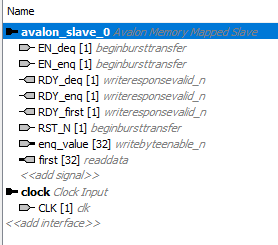
\includegraphics{images/Example1BeforeOranization.png} \\
This is unfortunately easier said than done. There are few options of assigning those wires, but neither of them perfect. Firstly we will need to choose a type of interface those will represent. We have over 30 options to chose from, but most of them are variants of larger protocols like AXI4. The only option that will make sense for us is Conduit, which basically meaningless bank canvas. We could create a conduit for each method but after consultation with my supervisor he recommended creating a conduit for each wire. So I did as he recommended, and this produces following set of interfaces. This requires quite a bit of manual work, listed bellow.
\begin{itemize}
    \item Create 8 new interfaces (QSys figured out what to do with clock wire on its own, so we have one for free) this includes giving them a name and assigning a reset signal.
    \item More each wire to its respective interface and change signal type of each wire to something generic like wire from type given to it as part of Avalon slave interface. 
\end{itemize}

\begin{figure}
    \caption{After assigning wires and Interfaces}
    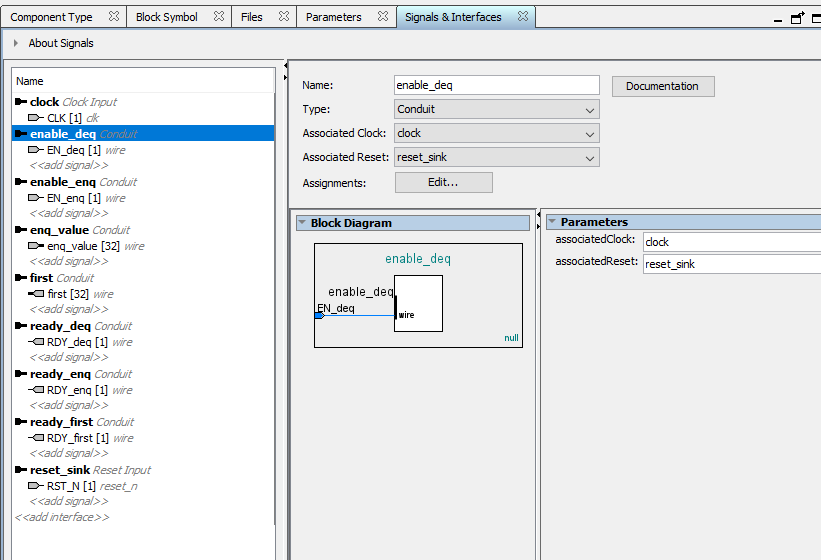
\includegraphics[width=\textwidth]{images/Example1AfterOrganization.png} \\
    \centering
\end{figure}

With all of those wires we can connect obvious things together like \verb!first! to \verb!enq_value! and clock signals, but then we run into a problem that with all wires that represent Ready-Enable micro protocol because we would like to enable enqueue in second queue only if both wires \verb!ready_deq! and \verb!ready_first! are high in the first queue, otherwise because we don't know how our FIFO is implemented we might run into a problem where we might get bugs(for example we lose data because we \verb!ready_deq! became high cycle faster than \verb!ready_first!, or in opposite scenario we would read stale/corrupted data). Unfortunately we can't create such logic using platform designer and one way of solving this would be to create special connector module that would do this logic(I'm going to come back later to explain why this approach might be infeasible in general case). 

\subsection{My tool}
Using my tool whole phase of importing and setting up wires can be skipped. Connecting is as simple as creating a new node connection node and selecting chosen FIFO's interface. Extending two connected FIFOs to three is as simple as adding one more FIFO and one more connection node.

\begin{figure}
    \caption{Three connected FIFOs using my tool}
    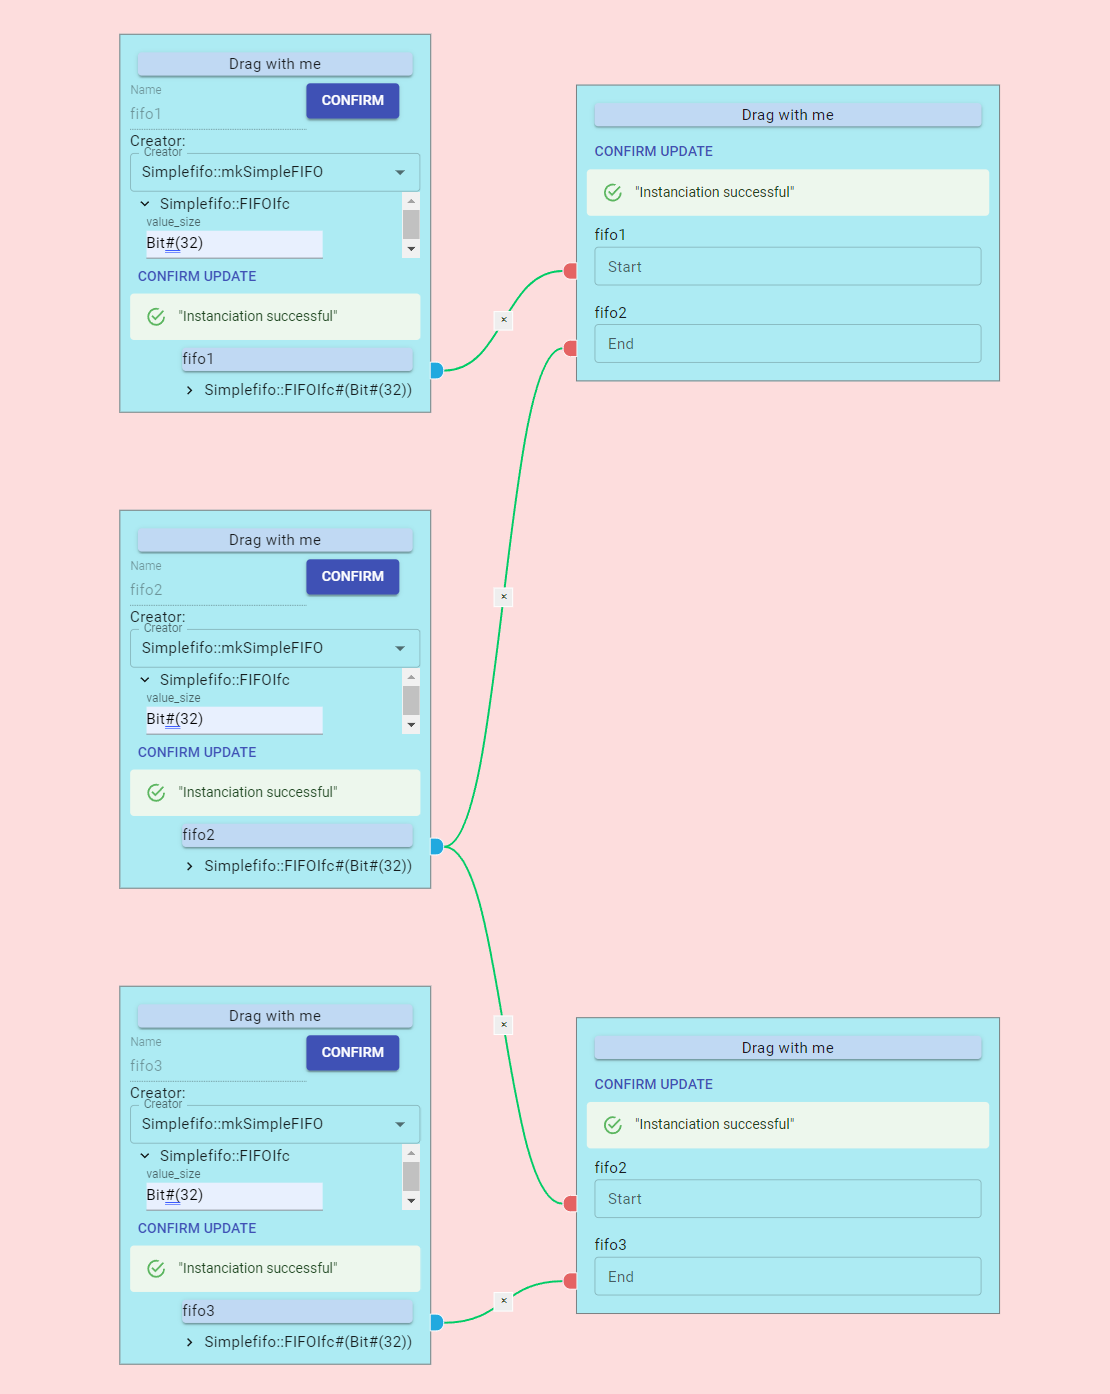
\includegraphics[width=0.7\textwidth]{images/Example1MySolution.png} \\
    \centering
\end{figure}

\subsection{Using text format to do same things and Qualitative metrics}
To count number of tokens I'm using following regexp \verb!(\w|\.)+!. This regexp will match sequences of alphanumerical characters with dots and underscores. (TODO draw graphs)
Raw numbers: 431 tokens to import FIFO, 347 for two connected FIFOs, and 415 for three connected FIFOs.
My solution: 31 for two connected FIFOs and 43 for three connected FIFOs.

\section{Example 2 - Simple System-on-Chip}
In this example we will create a simple system-on-chip (SOC) with one Flute core, memory module and fake interface with outside world, all connected by a bus. This example is designed to even out playing field by making all connections use AXI4 interface which is undestood by platform designer.

\subsection{Platform Designer}
Again we start with importing our modules. 
This time we need to import two of them, one for fake 16550 interface and one for flute core. 
As for memory module we will use one from QSys library to save time and effort.

Unfortunately platform designer can't figure out how to organize wires into interfaces like AXI4 master or AXI4 slave. 
So we need to do it manually. This wouldn't be so painful if not for the fact that we need to set type of each wire according to it's name(for example \verb!cpu_imem_master_awready! has type \verb!awready!). Each of those AXI4 interfaces has 37 wires, and if we account for all other interfaces of Flute core we get 150 wires that individually need to be assigned to interfaces. Similarly, our fake 16550 interfaces also uses 40 wires in total. When assigning this through GUI it took me around 16 minutes to click through all the assignments. (For context tools like Xilinx Vivado have heuristics that are able to do a lot of this automatically, but my understanding is that still this works only for certain known interfaces)
\\
\begin{figure}
    \caption{Connected Sys-on-Chip using Platform designer}
    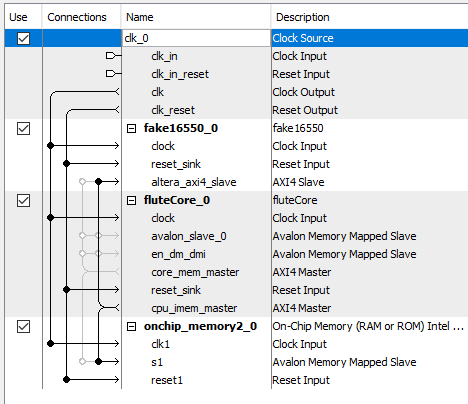
\includegraphics[width=0.7\textwidth]{images/Example2QSys.png} \\
    \centering
\end{figure}
After initial pain of importing modules we arrive at the place where Platform designer shines. It is able to show possible connections between AXI4 masters and slaves, on a two 2 grid-like layout. Then connecting two together is as simple as clicking cross-section of two wires on the screen.  

\subsection{My tool}
Again using my tool we don't need to do anything to import modules, as all the typing information is provided by the package. To connect those together we create a special bus node, select function for creating a bus, select number of masters and slaves, then assign each accordingly. While I'm unable to show nice 2d grid of possible connections, I have two-stage autocompletion. Stage 1 autocompletion becomes available after user selects function to create a bus. Such functions can be polymorphic, so I show all interfaces that might be valid individually, but not necessarily together. Stage 2 autocompletion becomes available after user selects at least one master and at least one slave, and clicks confirm update. After that bus is locked to specific type of masters and slaves and autocompletion narrows to show only masters and slaves that will work together.
\begin{figure}
    \caption{Connected Sys-on-Chip using my tool}
    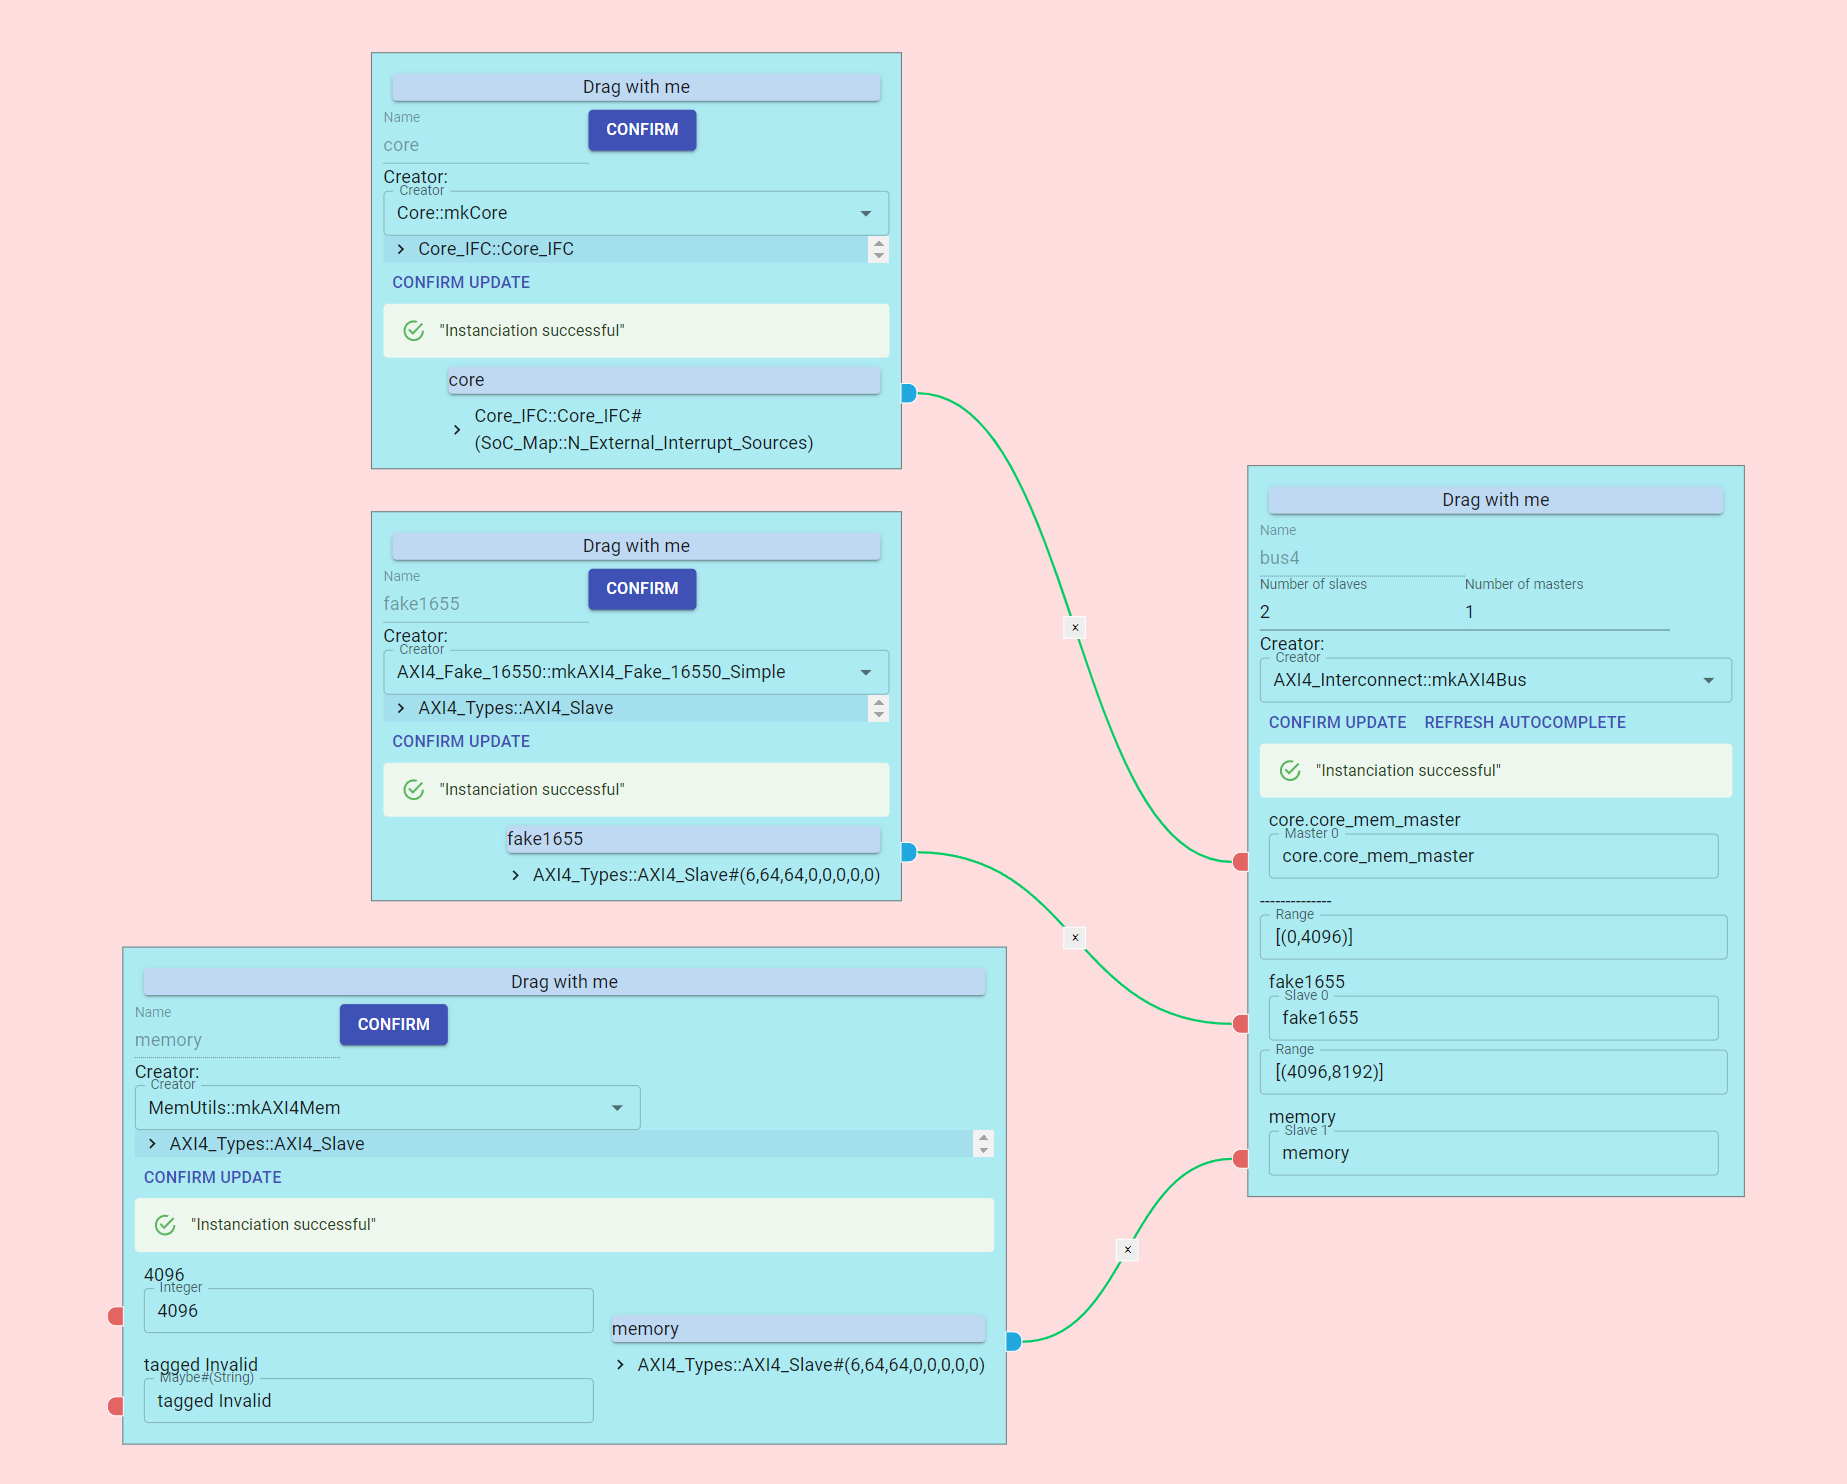
\includegraphics[width=0.8\textwidth]{images/Example2MySolution.png} \\
    \centering
\end{figure}

\subsection{Other differences}
There is a number of subtle differences that are worth talking about, but were not pronounced by this example.
\\
Platform designer has ability to automatically convert between AXI4 interfaces and Avalon ones, and also within those families it allows for some degree of flexibility when parameters don't match exactly.
When I create busses I'm limited by typing system, and way functions for creating buses were defined. Therefore, if user wants to do similar conversions they would need to use some functions and perform those conversions by themselves.
\\
Another slight difference is the fact that in Platform designer, each master has its own bus, and while slaves can be connected to any number of masters they need to be connected individually. 
\section{Example 3 - Working AXI4 masters and slaves}
This example 
\end{document}
